\documentclass[1p]{elsarticle_modified}
%\bibliographystyle{elsarticle-num}

%\usepackage[colorlinks]{hyperref}
%\usepackage{abbrmath_seonhwa} %\Abb, \Ascr, \Acal ,\Abf, \Afrak
\usepackage{amsfonts}
\usepackage{amssymb}
\usepackage{amsmath}
\usepackage{amsthm}
\usepackage{scalefnt}
\usepackage{amsbsy}
\usepackage{kotex}
\usepackage{caption}
\usepackage{subfig}
\usepackage{color}
\usepackage{graphicx}
\usepackage{xcolor} %% white, black, red, green, blue, cyan, magenta, yellow
\usepackage{float}
\usepackage{setspace}
\usepackage{hyperref}

\usepackage{tikz}
\usetikzlibrary{arrows}

\usepackage{multirow}
\usepackage{array} % fixed length table
\usepackage{hhline}

%%%%%%%%%%%%%%%%%%%%%
\makeatletter
\renewcommand*\env@matrix[1][\arraystretch]{%
	\edef\arraystretch{#1}%
	\hskip -\arraycolsep
	\let\@ifnextchar\new@ifnextchar
	\array{*\c@MaxMatrixCols c}}
\makeatother %https://tex.stackexchange.com/questions/14071/how-can-i-increase-the-line-spacing-in-a-matrix
%%%%%%%%%%%%%%%

\usepackage[normalem]{ulem}

\newcommand{\msout}[1]{\ifmmode\text{\sout{\ensuremath{#1}}}\else\sout{#1}\fi}
%SOURCE: \msout is \stkout macro in https://tex.stackexchange.com/questions/20609/strikeout-in-math-mode

\newcommand{\cancel}[1]{
	\ifmmode
	{\color{red}\msout{#1}}
	\else
	{\color{red}\sout{#1}}
	\fi
}

\newcommand{\add}[1]{
	{\color{blue}\uwave{#1}}
}

\newcommand{\replace}[2]{
	\ifmmode
	{\color{red}\msout{#1}}{\color{blue}\uwave{#2}}
	\else
	{\color{red}\sout{#1}}{\color{blue}\uwave{#2}}
	\fi
}

\newcommand{\Sol}{\mathcal{S}} %segment
\newcommand{\D}{D} %diagram
\newcommand{\A}{\mathcal{A}} %arc


%%%%%%%%%%%%%%%%%%%%%%%%%%%%%5 test

\def\sl{\operatorname{\textup{SL}}(2,\Cbb)}
\def\psl{\operatorname{\textup{PSL}}(2,\Cbb)}
\def\quan{\mkern 1mu \triangleright \mkern 1mu}

\theoremstyle{definition}
\newtheorem{thm}{Theorem}[section]
\newtheorem{prop}[thm]{Proposition}
\newtheorem{lem}[thm]{Lemma}
\newtheorem{ques}[thm]{Question}
\newtheorem{cor}[thm]{Corollary}
\newtheorem{defn}[thm]{Definition}
\newtheorem{exam}[thm]{Example}
\newtheorem{rmk}[thm]{Remark}
\newtheorem{alg}[thm]{Algorithm}

\newcommand{\I}{\sqrt{-1}}
\begin{document}

%\begin{frontmatter}
%
%\title{Boundary parabolic representations of knots up to 8 crossings}
%
%%% Group authors per affiliation:
%\author{Yunhi Cho} 
%\address{Department of Mathematics, University of Seoul, Seoul, Korea}
%\ead{yhcho@uos.ac.kr}
%
%
%\author{Seonhwa Kim} %\fnref{s_kim}}
%\address{Center for Geometry and Physics, Institute for Basic Science, Pohang, 37673, Korea}
%\ead{ryeona17@ibs.re.kr}
%
%\author{Hyuk Kim}
%\address{Department of Mathematical Sciences, Seoul National University, Seoul 08826, Korea}
%\ead{hyukkim@snu.ac.kr}
%
%\author{Seokbeom Yoon}
%\address{Department of Mathematical Sciences, Seoul National University, Seoul, 08826,  Korea}
%\ead{sbyoon15@snu.ac.kr}
%
%\begin{abstract}
%We find all boundary parabolic representation of knots up to 8 crossings.
%
%\end{abstract}
%\begin{keyword}
%    \MSC[2010] 57M25 
%\end{keyword}
%
%\end{frontmatter}

%\linenumbers
%\tableofcontents
%
\newcommand\colored[1]{\textcolor{white}{\rule[-0.35ex]{0.8em}{1.4ex}}\kern-0.8em\color{red} #1}%
%\newcommand\colored[1]{\textcolor{white}{ #1}\kern-2.17ex	\textcolor{white}{ #1}\kern-1.81ex	\textcolor{white}{ #1}\kern-2.15ex\color{red}#1	}

{\Large $\underline{12n_{0412}~(K12n_{0412})}$}

\setlength{\tabcolsep}{10pt}
\renewcommand{\arraystretch}{1.6}
\vspace{1cm}\begin{tabular}{m{100pt}>{\centering\arraybackslash}m{274pt}}
\multirow{5}{120pt}{
	\centering
	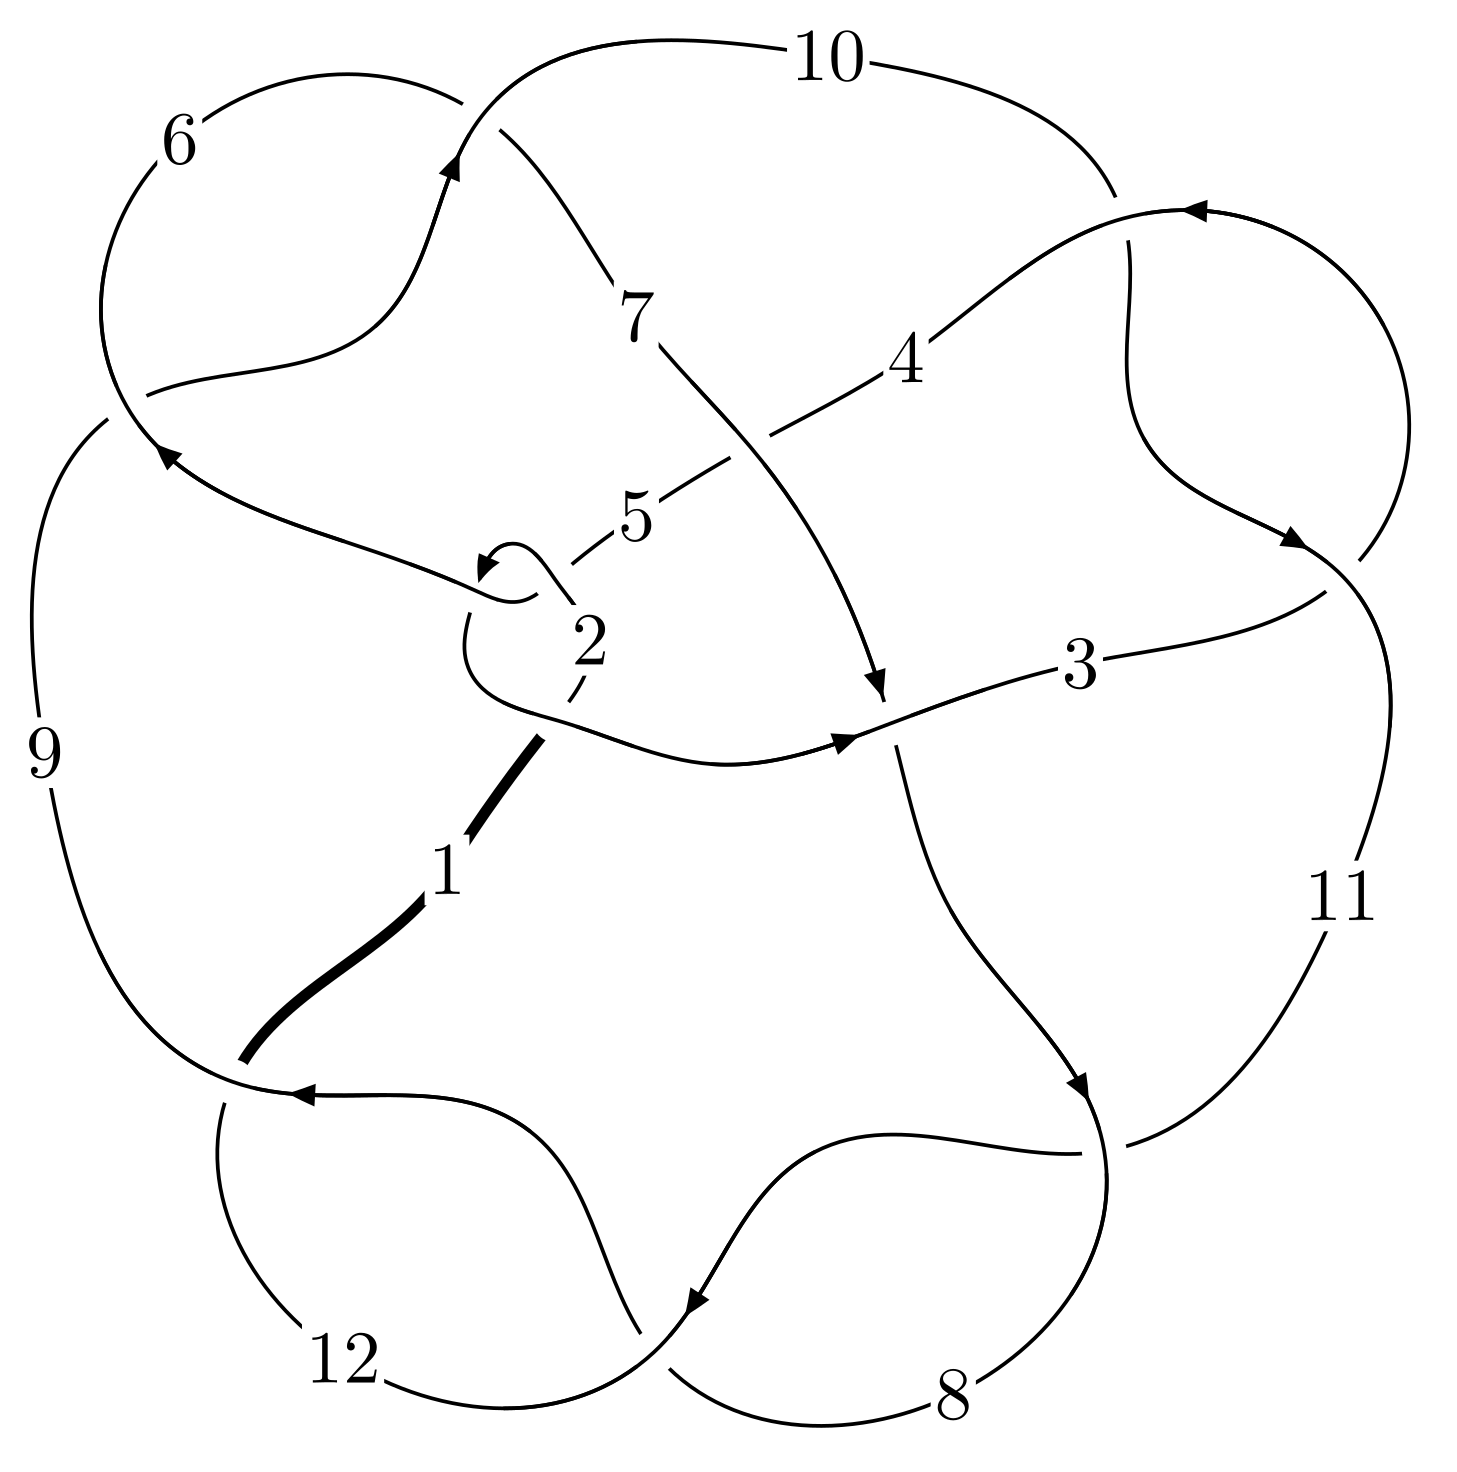
\includegraphics[width=112pt]{../../../GIT/diagram.site/Diagrams/png/2501_12n_0412.png}\\
\ \ \ A knot diagram\footnotemark}&
\allowdisplaybreaks
\textbf{Linearized knot diagam} \\
\cline{2-2}
 &
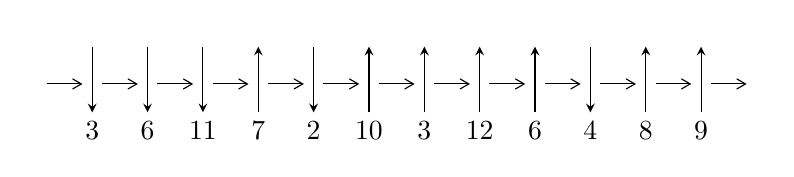
\begin{tikzpicture}[x=20pt, y=17pt]
	% nodes
	\node (C0) at (0, 0) {};
	\node (C1) at (1, 0) {};
	\node (C1U) at (1, +1) {};
	\node (C1D) at (1, -1) {3};

	\node (C2) at (2, 0) {};
	\node (C2U) at (2, +1) {};
	\node (C2D) at (2, -1) {6};

	\node (C3) at (3, 0) {};
	\node (C3U) at (3, +1) {};
	\node (C3D) at (3, -1) {11};

	\node (C4) at (4, 0) {};
	\node (C4U) at (4, +1) {};
	\node (C4D) at (4, -1) {7};

	\node (C5) at (5, 0) {};
	\node (C5U) at (5, +1) {};
	\node (C5D) at (5, -1) {2};

	\node (C6) at (6, 0) {};
	\node (C6U) at (6, +1) {};
	\node (C6D) at (6, -1) {10};

	\node (C7) at (7, 0) {};
	\node (C7U) at (7, +1) {};
	\node (C7D) at (7, -1) {3};

	\node (C8) at (8, 0) {};
	\node (C8U) at (8, +1) {};
	\node (C8D) at (8, -1) {12};

	\node (C9) at (9, 0) {};
	\node (C9U) at (9, +1) {};
	\node (C9D) at (9, -1) {6};

	\node (C10) at (10, 0) {};
	\node (C10U) at (10, +1) {};
	\node (C10D) at (10, -1) {4};

	\node (C11) at (11, 0) {};
	\node (C11U) at (11, +1) {};
	\node (C11D) at (11, -1) {8};

	\node (C12) at (12, 0) {};
	\node (C12U) at (12, +1) {};
	\node (C12D) at (12, -1) {9};
	\node (C13) at (13, 0) {};

	% arrows
	\draw[->,>={angle 60}]
	(C0) edge (C1) (C1) edge (C2) (C2) edge (C3) (C3) edge (C4) (C4) edge (C5) (C5) edge (C6) (C6) edge (C7) (C7) edge (C8) (C8) edge (C9) (C9) edge (C10) (C10) edge (C11) (C11) edge (C12) (C12) edge (C13) ;	\draw[->,>=stealth]
	(C1U) edge (C1D) (C2U) edge (C2D) (C3U) edge (C3D) (C4D) edge (C4U) (C5U) edge (C5D) (C6D) edge (C6U) (C7D) edge (C7U) (C8D) edge (C8U) (C9D) edge (C9U) (C10U) edge (C10D) (C11D) edge (C11U) (C12D) edge (C12U) ;
	\end{tikzpicture} \\
\hhline{~~} \\& 
\textbf{Solving Sequence} \\ \cline{2-2} 
 &
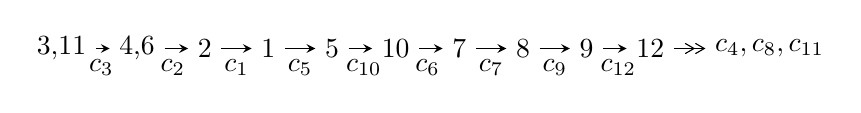
\begin{tikzpicture}[x=23pt, y=7pt]
	% node
	\node (A0) at (-1/8, 0) {3,11};
	\node (A1) at (17/16, 0) {4,6};
	\node (A2) at (17/8, 0) {2};
	\node (A3) at (25/8, 0) {1};
	\node (A4) at (33/8, 0) {5};
	\node (A5) at (41/8, 0) {10};
	\node (A6) at (49/8, 0) {7};
	\node (A7) at (57/8, 0) {8};
	\node (A8) at (65/8, 0) {9};
	\node (A9) at (73/8, 0) {12};
	\node (C1) at (1/2, -1) {$c_{3}$};
	\node (C2) at (13/8, -1) {$c_{2}$};
	\node (C3) at (21/8, -1) {$c_{1}$};
	\node (C4) at (29/8, -1) {$c_{5}$};
	\node (C5) at (37/8, -1) {$c_{10}$};
	\node (C6) at (45/8, -1) {$c_{6}$};
	\node (C7) at (53/8, -1) {$c_{7}$};
	\node (C8) at (61/8, -1) {$c_{9}$};
	\node (C9) at (69/8, -1) {$c_{12}$};
	\node (A10) at (11, 0) {$c_{4},c_{8},c_{11}$};

	% edge
	\draw[->,>=stealth]	
	(A0) edge (A1) (A1) edge (A2) (A2) edge (A3) (A3) edge (A4) (A4) edge (A5) (A5) edge (A6) (A6) edge (A7) (A7) edge (A8) (A8) edge (A9) ;
	\draw[->>,>={angle 60}]	
	(A9) edge (A10);
\end{tikzpicture} \\ 

\end{tabular} \\

\footnotetext{
The image of knot diagram is generated by the software ``\textbf{Draw programme}" developed by Andrew Bartholomew(\url{http://www.layer8.co.uk/maths/draw/index.htm\#Running-draw}), where we modified some parts for our purpose(\url{https://github.com/CATsTAILs/LinksPainter}).
}\phantom \\ \newline 
\centering \textbf{Ideals for irreducible components\footnotemark of $X_{\text{par}}$} 
 
\begin{align*}
I^u_{1}&=\langle 
-1.84897\times10^{24} u^{44}-2.54096\times10^{24} u^{43}+\cdots+3.58820\times10^{24} b+5.26379\times10^{24},\\
\phantom{I^u_{1}}&\phantom{= \langle  }1.76545\times10^{23} u^{44}+3.27410\times10^{23} u^{43}+\cdots+4.32313\times10^{22} a+2.31306\times10^{23},\;u^{45}+2 u^{44}+\cdots+8 u-1\rangle \\
I^u_{2}&=\langle 
- u^{12}+u^{11}-6 u^{10}+5 u^9-12 u^8+9 u^7-6 u^6+6 u^5+6 u^4+3 u^2+b- u-1,\\
\phantom{I^u_{2}}&\phantom{= \langle  }2 u^{12}- u^{11}+11 u^{10}-4 u^9+20 u^8-6 u^7+7 u^6-6 u^5-14 u^4-7 u^3-10 u^2+a-4 u-2,\\
\phantom{I^u_{2}}&\phantom{= \langle  }u^{13}- u^{12}+7 u^{11}-6 u^{10}+18 u^9-14 u^8+18 u^7-15 u^6-6 u^4-9 u^3+u^2-2 u+1\rangle \\
I^u_{3}&=\langle 
- u^2+b,\;a-1,\;u^4- u^3+2 u^2-2 u+1\rangle \\
I^u_{4}&=\langle 
b-1,\;a-1,\;u+1\rangle \\
\\
\end{align*}
\raggedright * 4 irreducible components of $\dim_{\mathbb{C}}=0$, with total 63 representations.\\
\footnotetext{All coefficients of polynomials are rational numbers. But the coefficients are sometimes approximated in decimal forms when there is not enough margin.}
\newpage
\renewcommand{\arraystretch}{1}
\centering \section*{I. $I^u_{1}= \langle -1.85\times10^{24} u^{44}-2.54\times10^{24} u^{43}+\cdots+3.59\times10^{24} b+5.26\times10^{24},\;1.77\times10^{23} u^{44}+3.27\times10^{23} u^{43}+\cdots+4.32\times10^{22} a+2.31\times10^{23},\;u^{45}+2 u^{44}+\cdots+8 u-1 \rangle$}
\flushleft \textbf{(i) Arc colorings}\\
\begin{tabular}{m{7pt} m{180pt} m{7pt} m{180pt} }
\flushright $a_{3}=$&$\begin{pmatrix}1\\0\end{pmatrix}$ \\
\flushright $a_{11}=$&$\begin{pmatrix}0\\u\end{pmatrix}$ \\
\flushright $a_{4}=$&$\begin{pmatrix}1\\u^2\end{pmatrix}$ \\
\flushright $a_{6}=$&$\begin{pmatrix}-4.08374 u^{44}-7.57346 u^{43}+\cdots-218.809 u-5.35044\\0.515292 u^{44}+0.708144 u^{43}+\cdots+6.15932 u-1.46697\end{pmatrix}$ \\
\flushright $a_{2}=$&$\begin{pmatrix}2.87916 u^{44}+5.44800 u^{43}+\cdots+83.3782 u-24.3626\\-1.12930 u^{44}-2.18153 u^{43}+\cdots-42.3482 u+3.36146\end{pmatrix}$ \\
\flushright $a_{1}=$&$\begin{pmatrix}1.74987 u^{44}+3.26646 u^{43}+\cdots+41.0300 u-21.0011\\-1.12930 u^{44}-2.18153 u^{43}+\cdots-42.3482 u+3.36146\end{pmatrix}$ \\
\flushright $a_{5}=$&$\begin{pmatrix}2.61866 u^{44}+4.36589 u^{43}+\cdots+46.2417 u-15.9362\\-2.70869 u^{44}-4.60335 u^{43}+\cdots-87.4930 u+7.47428\end{pmatrix}$ \\
\flushright $a_{10}=$&$\begin{pmatrix}u\\u^3+u\end{pmatrix}$ \\
\flushright $a_{7}=$&$\begin{pmatrix}-3.56455 u^{44}-6.80670 u^{43}+\cdots-206.802 u-6.30618\\1.00518 u^{44}+1.76026 u^{43}+\cdots+20.8578 u-2.69432\end{pmatrix}$ \\
\flushright $a_{8}=$&$\begin{pmatrix}-2.55937 u^{44}-5.04644 u^{43}+\cdots-185.944 u-9.00050\\1.00518 u^{44}+1.76026 u^{43}+\cdots+20.8578 u-2.69432\end{pmatrix}$ \\
\flushright $a_{9}=$&$\begin{pmatrix}-1.96341 u^{44}-3.93259 u^{43}+\cdots-196.681 u-18.9609\\-1.50697 u^{44}-2.36388 u^{43}+\cdots-62.6688 u+4.32930\end{pmatrix}$ \\
\flushright $a_{12}=$&$\begin{pmatrix}4.25404 u^{44}+7.98425 u^{43}+\cdots+282.601 u+14.5444\\-0.0622841 u^{44}-1.08570 u^{43}+\cdots+10.5596 u+0.527328\end{pmatrix}$\\&\end{tabular}
\flushleft \textbf{(ii) Obstruction class $= -1$}\\~\\
\flushleft \textbf{(iii) Cusp Shapes $= \frac{20998050926369734752976211}{3588196003166548679987327} u^{44}+\frac{37483540873690423560378912}{3588196003166548679987327} u^{43}+\cdots+\frac{1213475306781566067904042936}{3588196003166548679987327} u-\frac{19958410998607784963592834}{3588196003166548679987327}$}\\~\\
\newpage\renewcommand{\arraystretch}{1}
\flushleft \textbf{(iv) u-Polynomials at the component}\newline \\
\begin{tabular}{m{50pt}|m{274pt}}
Crossings & \hspace{64pt}u-Polynomials at each crossing \\
\hline $$\begin{aligned}c_{1}\end{aligned}$$&$\begin{aligned}
&u^{45}+48 u^{44}+\cdots+584 u+1
\end{aligned}$\\
\hline $$\begin{aligned}c_{2},c_{5}\end{aligned}$$&$\begin{aligned}
&u^{45}+4 u^{44}+\cdots-42 u+1
\end{aligned}$\\
\hline $$\begin{aligned}c_{3},c_{10}\end{aligned}$$&$\begin{aligned}
&u^{45}+2 u^{44}+\cdots+8 u-1
\end{aligned}$\\
\hline $$\begin{aligned}c_{4}\end{aligned}$$&$\begin{aligned}
&u^{45}+9 u^{44}+\cdots+1549 u+311
\end{aligned}$\\
\hline $$\begin{aligned}c_{6},c_{9}\end{aligned}$$&$\begin{aligned}
&u^{45}-4 u^{44}+\cdots-15 u-1
\end{aligned}$\\
\hline $$\begin{aligned}c_{7}\end{aligned}$$&$\begin{aligned}
&u^{45}+3 u^{44}+\cdots-8958 u+563
\end{aligned}$\\
\hline $$\begin{aligned}c_{8},c_{11},c_{12}\end{aligned}$$&$\begin{aligned}
&u^{45}+4 u^{44}+\cdots+58 u+28
\end{aligned}$\\
\hline
\end{tabular}\\~\\
\newpage\renewcommand{\arraystretch}{1}
\flushleft \textbf{(v) Riley Polynomials at the component}\newline \\
\begin{tabular}{m{50pt}|m{274pt}}
Crossings & \hspace{64pt}Riley Polynomials at each crossing \\
\hline $$\begin{aligned}c_{1}\end{aligned}$$&$\begin{aligned}
&y^{45}-96 y^{44}+\cdots+113992 y-1
\end{aligned}$\\
\hline $$\begin{aligned}c_{2},c_{5}\end{aligned}$$&$\begin{aligned}
&y^{45}-48 y^{44}+\cdots+584 y-1
\end{aligned}$\\
\hline $$\begin{aligned}c_{3},c_{10}\end{aligned}$$&$\begin{aligned}
&y^{45}+42 y^{44}+\cdots+252 y-1
\end{aligned}$\\
\hline $$\begin{aligned}c_{4}\end{aligned}$$&$\begin{aligned}
&y^{45}+9 y^{44}+\cdots-3165011 y-96721
\end{aligned}$\\
\hline $$\begin{aligned}c_{6},c_{9}\end{aligned}$$&$\begin{aligned}
&y^{45}-12 y^{44}+\cdots+105 y-1
\end{aligned}$\\
\hline $$\begin{aligned}c_{7}\end{aligned}$$&$\begin{aligned}
&y^{45}- y^{44}+\cdots+19794202 y-316969
\end{aligned}$\\
\hline $$\begin{aligned}c_{8},c_{11},c_{12}\end{aligned}$$&$\begin{aligned}
&y^{45}-36 y^{44}+\cdots-1060 y-784
\end{aligned}$\\
\hline
\end{tabular}\\~\\
\newpage\flushleft \textbf{(vi) Complex Volumes and Cusp Shapes}
$$\begin{array}{c|c|c}  
\text{Solutions to }I^u_{1}& \I (\text{vol} + \sqrt{-1}CS) & \text{Cusp shape}\\
 \hline 
\begin{aligned}
u &= \phantom{-}0.969825\phantom{ +0.000000I} \\
a &= \phantom{-}0.229176\phantom{ +0.000000I} \\
b &= \phantom{-}0.627201\phantom{ +0.000000I}\end{aligned}
 & \phantom{-}2.96038\phantom{ +0.000000I} & -2.69630\phantom{ +0.000000I} \\ \hline\begin{aligned}
u &= -0.927844 + 0.271505 I \\
a &= -1.041520 - 0.768905 I \\
b &= -1.52557 + 0.45145 I\end{aligned}
 & -4.45709 + 9.42399 I & \phantom{-}1.94019 - 6.31293 I \\ \hline\begin{aligned}
u &= -0.927844 - 0.271505 I \\
a &= -1.041520 + 0.768905 I \\
b &= -1.52557 - 0.45145 I\end{aligned}
 & -4.45709 - 9.42399 I & \phantom{-}1.94019 + 6.31293 I \\ \hline\begin{aligned}
u &= \phantom{-}0.845626 + 0.121557 I \\
a &= -1.42589 + 0.88397 I \\
b &= -1.59489 - 0.20003 I\end{aligned}
 & -8.64870 - 3.87589 I & -1.85841 + 2.88964 I \\ \hline\begin{aligned}
u &= \phantom{-}0.845626 - 0.121557 I \\
a &= -1.42589 - 0.88397 I \\
b &= -1.59489 + 0.20003 I\end{aligned}
 & -8.64870 + 3.87589 I & -1.85841 - 2.88964 I \\ \hline\begin{aligned}
u &= -0.164418 + 1.159280 I \\
a &= \phantom{-}0.703495 - 0.012931 I \\
b &= -0.763782 - 0.015983 I\end{aligned}
 & \phantom{-}1.53495 + 1.91036 I & \phantom{-0.000000 } 0 \\ \hline\begin{aligned}
u &= -0.164418 - 1.159280 I \\
a &= \phantom{-}0.703495 + 0.012931 I \\
b &= -0.763782 + 0.015983 I\end{aligned}
 & \phantom{-}1.53495 - 1.91036 I & \phantom{-0.000000 } 0 \\ \hline\begin{aligned}
u &= -0.669119 + 1.011720 I \\
a &= -0.065566 + 0.383511 I \\
b &= \phantom{-}1.37234 + 0.41380 I\end{aligned}
 & -2.27065 - 3.93661 I & \phantom{-0.000000 } 0 \\ \hline\begin{aligned}
u &= -0.669119 - 1.011720 I \\
a &= -0.065566 - 0.383511 I \\
b &= \phantom{-}1.37234 - 0.41380 I\end{aligned}
 & -2.27065 + 3.93661 I & \phantom{-0.000000 } 0 \\ \hline\begin{aligned}
u &= \phantom{-}0.433424 + 1.140140 I \\
a &= \phantom{-}0.033142 - 0.457634 I \\
b &= \phantom{-}1.53847 - 0.16157 I\end{aligned}
 & -5.53838 - 0.69987 I & \phantom{-0.000000 } 0\\
 \hline 
 \end{array}$$\newpage$$\begin{array}{c|c|c}  
\text{Solutions to }I^u_{1}& \I (\text{vol} + \sqrt{-1}CS) & \text{Cusp shape}\\
 \hline 
\begin{aligned}
u &= \phantom{-}0.433424 - 1.140140 I \\
a &= \phantom{-}0.033142 + 0.457634 I \\
b &= \phantom{-}1.53847 + 0.16157 I\end{aligned}
 & -5.53838 + 0.69987 I & \phantom{-0.000000 } 0 \\ \hline\begin{aligned}
u &= \phantom{-}0.664310 + 0.362711 I \\
a &= \phantom{-}0.328543 - 0.232382 I \\
b &= \phantom{-}0.261717 + 1.042650 I\end{aligned}
 & \phantom{-}1.25167 - 3.95167 I & \phantom{-}3.83579 + 7.35409 I \\ \hline\begin{aligned}
u &= \phantom{-}0.664310 - 0.362711 I \\
a &= \phantom{-}0.328543 + 0.232382 I \\
b &= \phantom{-}0.261717 - 1.042650 I\end{aligned}
 & \phantom{-}1.25167 + 3.95167 I & \phantom{-}3.83579 - 7.35409 I \\ \hline\begin{aligned}
u &= \phantom{-}0.186812 + 1.238700 I \\
a &= -0.67404 + 1.33349 I \\
b &= -0.0820505 - 0.0136120 I\end{aligned}
 & \phantom{-}4.44974 - 2.14104 I & \phantom{-0.000000 } 0 \\ \hline\begin{aligned}
u &= \phantom{-}0.186812 - 1.238700 I \\
a &= -0.67404 - 1.33349 I \\
b &= -0.0820505 + 0.0136120 I\end{aligned}
 & \phantom{-}4.44974 + 2.14104 I & \phantom{-0.000000 } 0 \\ \hline\begin{aligned}
u &= -0.277987 + 1.263490 I \\
a &= -0.29175 + 2.28733 I \\
b &= \phantom{-}1.44630 + 0.06917 I\end{aligned}
 & -0.68250 + 1.70775 I & \phantom{-0.000000 } 0 \\ \hline\begin{aligned}
u &= -0.277987 - 1.263490 I \\
a &= -0.29175 - 2.28733 I \\
b &= \phantom{-}1.44630 - 0.06917 I\end{aligned}
 & -0.68250 - 1.70775 I & \phantom{-0.000000 } 0 \\ \hline\begin{aligned}
u &= -0.042319 + 1.295400 I \\
a &= \phantom{-}1.92633 - 1.12849 I \\
b &= -1.43287 + 0.42714 I\end{aligned}
 & \phantom{-}1.71514 + 2.64308 I & \phantom{-0.000000 } 0 \\ \hline\begin{aligned}
u &= -0.042319 - 1.295400 I \\
a &= \phantom{-}1.92633 + 1.12849 I \\
b &= -1.43287 - 0.42714 I\end{aligned}
 & \phantom{-}1.71514 - 2.64308 I & \phantom{-0.000000 } 0 \\ \hline\begin{aligned}
u &= -0.698216 + 0.025057 I \\
a &= -2.07891 + 1.01497 I \\
b &= -1.51929 + 0.08671 I\end{aligned}
 & -4.51834 + 1.81580 I & -0.317984 - 1.183332 I\\
 \hline 
 \end{array}$$\newpage$$\begin{array}{c|c|c}  
\text{Solutions to }I^u_{1}& \I (\text{vol} + \sqrt{-1}CS) & \text{Cusp shape}\\
 \hline 
\begin{aligned}
u &= -0.698216 - 0.025057 I \\
a &= -2.07891 - 1.01497 I \\
b &= -1.51929 - 0.08671 I\end{aligned}
 & -4.51834 - 1.81580 I & -0.317984 + 1.183332 I \\ \hline\begin{aligned}
u &= \phantom{-}0.022131 + 1.309670 I \\
a &= -0.56784 - 1.95572 I \\
b &= \phantom{-}0.735072 + 0.094789 I\end{aligned}
 & \phantom{-}11.93010 - 0.31866 I & \phantom{-0.000000 } 0 \\ \hline\begin{aligned}
u &= \phantom{-}0.022131 - 1.309670 I \\
a &= -0.56784 + 1.95572 I \\
b &= \phantom{-}0.735072 - 0.094789 I\end{aligned}
 & \phantom{-}11.93010 + 0.31866 I & \phantom{-0.000000 } 0 \\ \hline\begin{aligned}
u &= -0.283028 + 1.297280 I \\
a &= \phantom{-}0.178492 + 0.638649 I \\
b &= \phantom{-}1.58589 - 0.07568 I\end{aligned}
 & -0.37999 + 5.35975 I & \phantom{-0.000000 } 0 \\ \hline\begin{aligned}
u &= -0.283028 - 1.297280 I \\
a &= \phantom{-}0.178492 - 0.638649 I \\
b &= \phantom{-}1.58589 + 0.07568 I\end{aligned}
 & -0.37999 - 5.35975 I & \phantom{-0.000000 } 0 \\ \hline\begin{aligned}
u &= -0.597996 + 0.198058 I \\
a &= \phantom{-}0.565513 + 0.398750 I \\
b &= \phantom{-}0.610778 - 0.503827 I\end{aligned}
 & -1.21115 + 0.91442 I & -3.60220 - 2.86568 I \\ \hline\begin{aligned}
u &= -0.597996 - 0.198058 I \\
a &= \phantom{-}0.565513 - 0.398750 I \\
b &= \phantom{-}0.610778 + 0.503827 I\end{aligned}
 & -1.21115 - 0.91442 I & -3.60220 + 2.86568 I \\ \hline\begin{aligned}
u &= \phantom{-}0.373344 + 1.342530 I \\
a &= \phantom{-}0.355758 - 0.038695 I \\
b &= -0.554848 + 0.011852 I\end{aligned}
 & \phantom{-}7.39338 - 4.75135 I & \phantom{-0.000000 } 0 \\ \hline\begin{aligned}
u &= \phantom{-}0.373344 - 1.342530 I \\
a &= \phantom{-}0.355758 + 0.038695 I \\
b &= -0.554848 - 0.011852 I\end{aligned}
 & \phantom{-}7.39338 + 4.75135 I & \phantom{-0.000000 } 0 \\ \hline\begin{aligned}
u &= \phantom{-}0.364735 + 1.347540 I \\
a &= -0.11146 - 1.99685 I \\
b &= \phantom{-}1.62752 + 0.23183 I\end{aligned}
 & -4.02855 - 8.22129 I & \phantom{-0.000000 } 0\\
 \hline 
 \end{array}$$\newpage$$\begin{array}{c|c|c}  
\text{Solutions to }I^u_{1}& \I (\text{vol} + \sqrt{-1}CS) & \text{Cusp shape}\\
 \hline 
\begin{aligned}
u &= \phantom{-}0.364735 - 1.347540 I \\
a &= -0.11146 + 1.99685 I \\
b &= \phantom{-}1.62752 - 0.23183 I\end{aligned}
 & -4.02855 + 8.22129 I & \phantom{-0.000000 } 0 \\ \hline\begin{aligned}
u &= -0.224203 + 1.388850 I \\
a &= -0.14008 - 1.68654 I \\
b &= -0.683694 + 1.023800 I\end{aligned}
 & \phantom{-}3.89960 + 3.89681 I & \phantom{-0.000000 } 0 \\ \hline\begin{aligned}
u &= -0.224203 - 1.388850 I \\
a &= -0.14008 + 1.68654 I \\
b &= -0.683694 - 1.023800 I\end{aligned}
 & \phantom{-}3.89960 - 3.89681 I & \phantom{-0.000000 } 0 \\ \hline\begin{aligned}
u &= -0.42343 + 1.35553 I \\
a &= -0.257759 - 1.007550 I \\
b &= -0.974975 + 0.080869 I\end{aligned}
 & \phantom{-}6.02639 + 5.09405 I & \phantom{-0.000000 } 0 \\ \hline\begin{aligned}
u &= -0.42343 - 1.35553 I \\
a &= -0.257759 + 1.007550 I \\
b &= -0.974975 - 0.080869 I\end{aligned}
 & \phantom{-}6.02639 - 5.09405 I & \phantom{-0.000000 } 0 \\ \hline\begin{aligned}
u &= \phantom{-}0.26016 + 1.44165 I \\
a &= -0.50945 + 1.62773 I \\
b &= -0.22976 - 1.42824 I\end{aligned}
 & \phantom{-}7.03160 - 7.34948 I & \phantom{-0.000000 } 0 \\ \hline\begin{aligned}
u &= \phantom{-}0.26016 - 1.44165 I \\
a &= -0.50945 - 1.62773 I \\
b &= -0.22976 + 1.42824 I\end{aligned}
 & \phantom{-}7.03160 + 7.34948 I & \phantom{-0.000000 } 0 \\ \hline\begin{aligned}
u &= -0.38297 + 1.43752 I \\
a &= -0.11849 + 1.78135 I \\
b &= \phantom{-}1.60904 - 0.50615 I\end{aligned}
 & \phantom{-}0.9685 + 14.1285 I & \phantom{-0.000000 } 0 \\ \hline\begin{aligned}
u &= -0.38297 - 1.43752 I \\
a &= -0.11849 - 1.78135 I \\
b &= \phantom{-}1.60904 + 0.50615 I\end{aligned}
 & \phantom{-}0.9685 - 14.1285 I & \phantom{-0.000000 } 0 \\ \hline\begin{aligned}
u &= \phantom{-}0.15138 + 1.55206 I \\
a &= \phantom{-}0.159781 + 1.093010 I \\
b &= -0.865603 - 0.853905 I\end{aligned}
 & \phantom{-}8.49461 - 3.13739 I & \phantom{-0.000000 } 0\\
 \hline 
 \end{array}$$\newpage$$\begin{array}{c|c|c}  
\text{Solutions to }I^u_{1}& \I (\text{vol} + \sqrt{-1}CS) & \text{Cusp shape}\\
 \hline 
\begin{aligned}
u &= \phantom{-}0.15138 - 1.55206 I \\
a &= \phantom{-}0.159781 - 1.093010 I \\
b &= -0.865603 + 0.853905 I\end{aligned}
 & \phantom{-}8.49461 + 3.13739 I & \phantom{-0.000000 } 0 \\ \hline\begin{aligned}
u &= \phantom{-}0.331161\phantom{ +0.000000I} \\
a &= \phantom{-}1.93794\phantom{ +0.000000I} \\
b &= -0.0592996\phantom{ +0.000000I}\end{aligned}
 & \phantom{-}0.981240\phantom{ +0.000000I} & \phantom{-}11.9230\phantom{ +0.000000I} \\ \hline\begin{aligned}
u &= -0.294649 + 0.018682 I \\
a &= \phantom{-}1.26352 + 2.17214 I \\
b &= \phantom{-}1.52527 - 0.31408 I\end{aligned}
 & -2.46259 + 1.58513 I & -5.29016 - 4.20356 I \\ \hline\begin{aligned}
u &= -0.294649 - 0.018682 I \\
a &= \phantom{-}1.26352 - 2.17214 I \\
b &= \phantom{-}1.52527 + 0.31408 I\end{aligned}
 & -2.46259 - 1.58513 I & -5.29016 + 4.20356 I \\ \hline\begin{aligned}
u &= \phantom{-}0.0675368\phantom{ +0.000000I} \\
a &= -22.6308\phantom{ +0.000000I} \\
b &= -0.738031\phantom{ +0.000000I}\end{aligned}
 & \phantom{-}7.70079\phantom{ +0.000000I} & \phantom{-}22.1050\phantom{ +0.000000I}\\
 \hline 
 \end{array}$$\newpage\newpage\renewcommand{\arraystretch}{1}
\centering \section*{II. $I^u_{2}= \langle - u^{12}+u^{11}+\cdots+b-1,\;2 u^{12}- u^{11}+\cdots+a-2,\;u^{13}- u^{12}+\cdots-2 u+1 \rangle$}
\flushleft \textbf{(i) Arc colorings}\\
\begin{tabular}{m{7pt} m{180pt} m{7pt} m{180pt} }
\flushright $a_{3}=$&$\begin{pmatrix}1\\0\end{pmatrix}$ \\
\flushright $a_{11}=$&$\begin{pmatrix}0\\u\end{pmatrix}$ \\
\flushright $a_{4}=$&$\begin{pmatrix}1\\u^2\end{pmatrix}$ \\
\flushright $a_{6}=$&$\begin{pmatrix}-2 u^{12}+u^{11}+\cdots+4 u+2\\u^{12}- u^{11}+6 u^{10}-5 u^9+12 u^8-9 u^7+6 u^6-6 u^5-6 u^4-3 u^2+u+1\end{pmatrix}$ \\
\flushright $a_{2}=$&$\begin{pmatrix}-2 u^{12}+2 u^{11}+\cdots-6 u-1\\u^{12}- u^{11}+5 u^{10}-4 u^9+7 u^8-5 u^7- u^6- u^5-5 u^4+u^3+2 u^2-1\end{pmatrix}$ \\
\flushright $a_{1}=$&$\begin{pmatrix}- u^{12}+u^{11}+\cdots-6 u-2\\u^{12}- u^{11}+5 u^{10}-4 u^9+7 u^8-5 u^7- u^6- u^5-5 u^4+u^3+2 u^2-1\end{pmatrix}$ \\
\flushright $a_{5}=$&$\begin{pmatrix}3 u^{12}-2 u^{11}+\cdots- u+3\\-3 u^{12}+3 u^{11}+\cdots+8 u^2-3 u\end{pmatrix}$ \\
\flushright $a_{10}=$&$\begin{pmatrix}u\\u^3+u\end{pmatrix}$ \\
\flushright $a_{7}=$&$\begin{pmatrix}-2 u^{12}+2 u^{11}+\cdots+3 u+2\\u^{12}-2 u^{11}+\cdots-4 u^2+2 u\end{pmatrix}$ \\
\flushright $a_{8}=$&$\begin{pmatrix}- u^{12}-5 u^{10}- u^9-8 u^8-3 u^7- u^6+8 u^4+7 u^3+6 u^2+5 u+2\\u^{12}-2 u^{11}+\cdots-4 u^2+2 u\end{pmatrix}$ \\
\flushright $a_{9}=$&$\begin{pmatrix}2 u^{12}-2 u^{11}+\cdots- u-5\\u^{12}- u^{11}+\cdots+2 u-1\end{pmatrix}$ \\
\flushright $a_{12}=$&$\begin{pmatrix}-2 u^{12}+2 u^{11}+\cdots+2 u+4\\u^{12}-2 u^{11}+\cdots+4 u-1\end{pmatrix}$\\&\end{tabular}
\flushleft \textbf{(ii) Obstruction class $= 1$}\\~\\
\flushleft \textbf{(iii) Cusp Shapes $= 4 u^{12}-7 u^{11}+29 u^{10}-36 u^9+73 u^8-64 u^7+69 u^6-36 u^5-4 u^4+5 u^3-37 u^2-5$}\\~\\
\newpage\renewcommand{\arraystretch}{1}
\flushleft \textbf{(iv) u-Polynomials at the component}\newline \\
\begin{tabular}{m{50pt}|m{274pt}}
Crossings & \hspace{64pt}u-Polynomials at each crossing \\
\hline $$\begin{aligned}c_{1}\end{aligned}$$&$\begin{aligned}
&u^{13}-13 u^{12}+\cdots+10 u-1
\end{aligned}$\\
\hline $$\begin{aligned}c_{2}\end{aligned}$$&$\begin{aligned}
&u^{13}+3 u^{12}+\cdots+5 u^2-1
\end{aligned}$\\
\hline $$\begin{aligned}c_{3}\end{aligned}$$&$\begin{aligned}
&u^{13}- u^{12}+\cdots-2 u+1
\end{aligned}$\\
\hline $$\begin{aligned}c_{4}\end{aligned}$$&$\begin{aligned}
&u^{13}-4 u^{11}+\cdots+9 u+1
\end{aligned}$\\
\hline $$\begin{aligned}c_{5}\end{aligned}$$&$\begin{aligned}
&u^{13}-3 u^{12}+\cdots-5 u^2+1
\end{aligned}$\\
\hline $$\begin{aligned}c_{6}\end{aligned}$$&$\begin{aligned}
&u^{13}-3 u^{12}+5 u^{10}- u^8-5 u^7-2 u^6+6 u^5- u^3- u^2- u+1
\end{aligned}$\\
\hline $$\begin{aligned}c_{7}\end{aligned}$$&$\begin{aligned}
&u^{13}-7 u^{11}+\cdots+2 u+1
\end{aligned}$\\
\hline $$\begin{aligned}c_{8}\end{aligned}$$&$\begin{aligned}
&u^{13}-8 u^{11}+\cdots+6 u^2-1
\end{aligned}$\\
\hline $$\begin{aligned}c_{9}\end{aligned}$$&$\begin{aligned}
&u^{13}+3 u^{12}-5 u^{10}+u^8-5 u^7+2 u^6+6 u^5- u^3+u^2- u-1
\end{aligned}$\\
\hline $$\begin{aligned}c_{10}\end{aligned}$$&$\begin{aligned}
&u^{13}+u^{12}+\cdots-2 u-1
\end{aligned}$\\
\hline $$\begin{aligned}c_{11},c_{12}\end{aligned}$$&$\begin{aligned}
&u^{13}-8 u^{11}+\cdots-6 u^2+1
\end{aligned}$\\
\hline
\end{tabular}\\~\\
\newpage\renewcommand{\arraystretch}{1}
\flushleft \textbf{(v) Riley Polynomials at the component}\newline \\
\begin{tabular}{m{50pt}|m{274pt}}
Crossings & \hspace{64pt}Riley Polynomials at each crossing \\
\hline $$\begin{aligned}c_{1}\end{aligned}$$&$\begin{aligned}
&y^{13}-21 y^{12}+\cdots+18 y-1
\end{aligned}$\\
\hline $$\begin{aligned}c_{2},c_{5}\end{aligned}$$&$\begin{aligned}
&y^{13}-13 y^{12}+\cdots+10 y-1
\end{aligned}$\\
\hline $$\begin{aligned}c_{3},c_{10}\end{aligned}$$&$\begin{aligned}
&y^{13}+13 y^{12}+\cdots+2 y-1
\end{aligned}$\\
\hline $$\begin{aligned}c_{4}\end{aligned}$$&$\begin{aligned}
&y^{13}-8 y^{12}+\cdots+31 y-1
\end{aligned}$\\
\hline $$\begin{aligned}c_{6},c_{9}\end{aligned}$$&$\begin{aligned}
&y^{13}-9 y^{12}+\cdots+3 y-1
\end{aligned}$\\
\hline $$\begin{aligned}c_{7}\end{aligned}$$&$\begin{aligned}
&y^{13}-14 y^{12}+\cdots+44 y-1
\end{aligned}$\\
\hline $$\begin{aligned}c_{8},c_{11},c_{12}\end{aligned}$$&$\begin{aligned}
&y^{13}-16 y^{12}+\cdots+12 y-1
\end{aligned}$\\
\hline
\end{tabular}\\~\\
\newpage\flushleft \textbf{(vi) Complex Volumes and Cusp Shapes}
$$\begin{array}{c|c|c}  
\text{Solutions to }I^u_{2}& \I (\text{vol} + \sqrt{-1}CS) & \text{Cusp shape}\\
 \hline 
\begin{aligned}
u &= \phantom{-}1.07246\phantom{ +0.000000I} \\
a &= \phantom{-}0.492294\phantom{ +0.000000I} \\
b &= \phantom{-}0.465079\phantom{ +0.000000I}\end{aligned}
 & \phantom{-}3.43265\phantom{ +0.000000I} & \phantom{-}15.5060\phantom{ +0.000000I} \\ \hline\begin{aligned}
u &= -0.034598 + 1.249270 I \\
a &= \phantom{-}1.56218 - 1.13850 I \\
b &= -1.74571 + 0.26973 I\end{aligned}
 & \phantom{-}0.86628 + 1.87846 I & \phantom{-}2.04855 - 1.94061 I \\ \hline\begin{aligned}
u &= -0.034598 - 1.249270 I \\
a &= \phantom{-}1.56218 + 1.13850 I \\
b &= -1.74571 - 0.26973 I\end{aligned}
 & \phantom{-}0.86628 - 1.87846 I & \phantom{-}2.04855 + 1.94061 I \\ \hline\begin{aligned}
u &= -0.686240\phantom{ +0.000000I} \\
a &= \phantom{-}1.32157\phantom{ +0.000000I} \\
b &= \phantom{-}0.679844\phantom{ +0.000000I}\end{aligned}
 & \phantom{-}0.244931\phantom{ +0.000000I} & -2.02350\phantom{ +0.000000I} \\ \hline\begin{aligned}
u &= \phantom{-}0.131294 + 1.356980 I \\
a &= \phantom{-}0.02881 + 1.98048 I \\
b &= -1.022270 - 0.441982 I\end{aligned}
 & \phantom{-}11.95140 - 1.70968 I & \phantom{-}8.67976 + 4.17356 I \\ \hline\begin{aligned}
u &= \phantom{-}0.131294 - 1.356980 I \\
a &= \phantom{-}0.02881 - 1.98048 I \\
b &= -1.022270 + 0.441982 I\end{aligned}
 & \phantom{-}11.95140 + 1.70968 I & \phantom{-}8.67976 - 4.17356 I \\ \hline\begin{aligned}
u &= -0.250597 + 1.356050 I \\
a &= -0.34025 - 1.50111 I \\
b &= -0.729247 + 0.638631 I\end{aligned}
 & \phantom{-}4.69917 + 3.36697 I & \phantom{-}7.60609 - 2.02916 I \\ \hline\begin{aligned}
u &= -0.250597 - 1.356050 I \\
a &= -0.34025 + 1.50111 I \\
b &= -0.729247 - 0.638631 I\end{aligned}
 & \phantom{-}4.69917 - 3.36697 I & \phantom{-}7.60609 + 2.02916 I \\ \hline\begin{aligned}
u &= -0.103530 + 0.564621 I \\
a &= \phantom{-}0.205252 + 1.185250 I \\
b &= \phantom{-}1.40513 + 0.23742 I\end{aligned}
 & -1.72775 - 1.40884 I & \phantom{-}6.28546 + 0.80673 I \\ \hline\begin{aligned}
u &= -0.103530 - 0.564621 I \\
a &= \phantom{-}0.205252 - 1.185250 I \\
b &= \phantom{-}1.40513 - 0.23742 I\end{aligned}
 & -1.72775 + 1.40884 I & \phantom{-}6.28546 - 0.80673 I\\
 \hline 
 \end{array}$$\newpage$$\begin{array}{c|c|c}  
\text{Solutions to }I^u_{2}& \I (\text{vol} + \sqrt{-1}CS) & \text{Cusp shape}\\
 \hline 
\begin{aligned}
u &= \phantom{-}0.39553 + 1.43394 I \\
a &= -0.341272 + 0.786047 I \\
b &= -0.429218 - 0.541128 I\end{aligned}
 & \phantom{-}8.26062 - 5.29255 I & \phantom{-}11.21555 + 5.90616 I \\ \hline\begin{aligned}
u &= \phantom{-}0.39553 - 1.43394 I \\
a &= -0.341272 - 0.786047 I \\
b &= -0.429218 + 0.541128 I\end{aligned}
 & \phantom{-}8.26062 + 5.29255 I & \phantom{-}11.21555 - 5.90616 I \\ \hline\begin{aligned}
u &= \phantom{-}0.337585\phantom{ +0.000000I} \\
a &= \phantom{-}4.95670\phantom{ +0.000000I} \\
b &= \phantom{-}0.897695\phantom{ +0.000000I}\end{aligned}
 & \phantom{-}7.44054\phantom{ +0.000000I} & -9.15310\phantom{ +0.000000I}\\
 \hline 
 \end{array}$$\newpage\newpage\renewcommand{\arraystretch}{1}
\centering \section*{III. $I^u_{3}= \langle - u^2+b,\;a-1,\;u^4- u^3+2 u^2-2 u+1 \rangle$}
\flushleft \textbf{(i) Arc colorings}\\
\begin{tabular}{m{7pt} m{180pt} m{7pt} m{180pt} }
\flushright $a_{3}=$&$\begin{pmatrix}1\\0\end{pmatrix}$ \\
\flushright $a_{11}=$&$\begin{pmatrix}0\\u\end{pmatrix}$ \\
\flushright $a_{4}=$&$\begin{pmatrix}1\\u^2\end{pmatrix}$ \\
\flushright $a_{6}=$&$\begin{pmatrix}1\\u^2\end{pmatrix}$ \\
\flushright $a_{2}=$&$\begin{pmatrix}- u^2+1\\- u^3+2 u^2-2 u+1\end{pmatrix}$ \\
\flushright $a_{1}=$&$\begin{pmatrix}- u^3+u^2-2 u+2\\- u^3+2 u^2-2 u+1\end{pmatrix}$ \\
\flushright $a_{5}=$&$\begin{pmatrix}- u^3+3 u^2-2 u+2\\u^3-2 u^2+3 u-1\end{pmatrix}$ \\
\flushright $a_{10}=$&$\begin{pmatrix}u\\u^3+u\end{pmatrix}$ \\
\flushright $a_{7}=$&$\begin{pmatrix}- u^2+1\\- u^3+2 u^2-2 u+1\end{pmatrix}$ \\
\flushright $a_{8}=$&$\begin{pmatrix}- u^3+u^2-2 u+2\\- u^3+2 u^2-2 u+1\end{pmatrix}$ \\
\flushright $a_{9}=$&$\begin{pmatrix}0\\u\end{pmatrix}$ \\
\flushright $a_{12}=$&$\begin{pmatrix}- u^3+u^2-2 u+2\\- u^3+2 u^2- u+1\end{pmatrix}$\\&\end{tabular}
\flushleft \textbf{(ii) Obstruction class $= -1$}\\~\\
\flushleft \textbf{(iii) Cusp Shapes $= 6$}\\~\\
\newpage\renewcommand{\arraystretch}{1}
\flushleft \textbf{(iv) u-Polynomials at the component}\newline \\
\begin{tabular}{m{50pt}|m{274pt}}
Crossings & \hspace{64pt}u-Polynomials at each crossing \\
\hline $$\begin{aligned}c_{1}\end{aligned}$$&$\begin{aligned}
&u^4+5 u^3+6 u^2-4 u+1
\end{aligned}$\\
\hline $$\begin{aligned}c_{2},c_{5}\end{aligned}$$&$\begin{aligned}
&u^4-3 u^3+2 u^2+1
\end{aligned}$\\
\hline $$\begin{aligned}c_{3},c_{6},c_{9}\\c_{10}\end{aligned}$$&$\begin{aligned}
&u^4- u^3+2 u^2-2 u+1
\end{aligned}$\\
\hline $$\begin{aligned}c_{4}\end{aligned}$$&$\begin{aligned}
&u^4+3 u^3+2 u^2+1
\end{aligned}$\\
\hline $$\begin{aligned}c_{7}\end{aligned}$$&$\begin{aligned}
&u^4-5 u^3+6 u^2+4 u+1
\end{aligned}$\\
\hline $$\begin{aligned}c_{8},c_{11},c_{12}\end{aligned}$$&$\begin{aligned}
&(u-1)^4
\end{aligned}$\\
\hline
\end{tabular}\\~\\
\newpage\renewcommand{\arraystretch}{1}
\flushleft \textbf{(v) Riley Polynomials at the component}\newline \\
\begin{tabular}{m{50pt}|m{274pt}}
Crossings & \hspace{64pt}Riley Polynomials at each crossing \\
\hline $$\begin{aligned}c_{1},c_{7}\end{aligned}$$&$\begin{aligned}
&y^4-13 y^3+78 y^2-4 y+1
\end{aligned}$\\
\hline $$\begin{aligned}c_{2},c_{4},c_{5}\end{aligned}$$&$\begin{aligned}
&y^4-5 y^3+6 y^2+4 y+1
\end{aligned}$\\
\hline $$\begin{aligned}c_{3},c_{6},c_{9}\\c_{10}\end{aligned}$$&$\begin{aligned}
&y^4+3 y^3+2 y^2+1
\end{aligned}$\\
\hline $$\begin{aligned}c_{8},c_{11},c_{12}\end{aligned}$$&$\begin{aligned}
&(y-1)^4
\end{aligned}$\\
\hline
\end{tabular}\\~\\
\newpage\flushleft \textbf{(vi) Complex Volumes and Cusp Shapes}
$$\begin{array}{c|c|c}  
\text{Solutions to }I^u_{3}& \I (\text{vol} + \sqrt{-1}CS) & \text{Cusp shape}\\
 \hline 
\begin{aligned}
u &= \phantom{-}0.621744 + 0.440597 I \\
a &= \phantom{-}1.00000\phantom{ +0.000000I} \\
b &= \phantom{-}0.192440 + 0.547877 I\end{aligned}
 & \phantom{-}1.64493\phantom{ +0.000000I} & \phantom{-}6.00000\phantom{ +0.000000I} \\ \hline\begin{aligned}
u &= \phantom{-}0.621744 - 0.440597 I \\
a &= \phantom{-}1.00000\phantom{ +0.000000I} \\
b &= \phantom{-}0.192440 - 0.547877 I\end{aligned}
 & \phantom{-}1.64493\phantom{ +0.000000I} & \phantom{-}6.00000\phantom{ +0.000000I} \\ \hline\begin{aligned}
u &= -0.121744 + 1.306620 I \\
a &= \phantom{-}1.00000\phantom{ +0.000000I} \\
b &= -1.69244 - 0.31815 I\end{aligned}
 & \phantom{-}1.64493\phantom{ +0.000000I} & \phantom{-}6.00000\phantom{ +0.000000I} \\ \hline\begin{aligned}
u &= -0.121744 - 1.306620 I \\
a &= \phantom{-}1.00000\phantom{ +0.000000I} \\
b &= -1.69244 + 0.31815 I\end{aligned}
 & \phantom{-}1.64493\phantom{ +0.000000I} & \phantom{-}6.00000\phantom{ +0.000000I}\\
 \hline 
 \end{array}$$\newpage\newpage\renewcommand{\arraystretch}{1}
\centering \section*{IV. $I^u_{4}= \langle b-1,\;a-1,\;u+1 \rangle$}
\flushleft \textbf{(i) Arc colorings}\\
\begin{tabular}{m{7pt} m{180pt} m{7pt} m{180pt} }
\flushright $a_{3}=$&$\begin{pmatrix}1\\0\end{pmatrix}$ \\
\flushright $a_{11}=$&$\begin{pmatrix}0\\-1\end{pmatrix}$ \\
\flushright $a_{4}=$&$\begin{pmatrix}1\\1\end{pmatrix}$ \\
\flushright $a_{6}=$&$\begin{pmatrix}1\\1\end{pmatrix}$ \\
\flushright $a_{2}=$&$\begin{pmatrix}0\\-1\end{pmatrix}$ \\
\flushright $a_{1}=$&$\begin{pmatrix}-1\\-1\end{pmatrix}$ \\
\flushright $a_{5}=$&$\begin{pmatrix}1\\0\end{pmatrix}$ \\
\flushright $a_{10}=$&$\begin{pmatrix}-1\\-2\end{pmatrix}$ \\
\flushright $a_{7}=$&$\begin{pmatrix}0\\-1\end{pmatrix}$ \\
\flushright $a_{8}=$&$\begin{pmatrix}-1\\-1\end{pmatrix}$ \\
\flushright $a_{9}=$&$\begin{pmatrix}0\\-1\end{pmatrix}$ \\
\flushright $a_{12}=$&$\begin{pmatrix}-1\\-2\end{pmatrix}$\\&\end{tabular}
\flushleft \textbf{(ii) Obstruction class $= -1$}\\~\\
\flushleft \textbf{(iii) Cusp Shapes $= 6$}\\~\\
\newpage\renewcommand{\arraystretch}{1}
\flushleft \textbf{(iv) u-Polynomials at the component}\newline \\
\begin{tabular}{m{50pt}|m{274pt}}
Crossings & \hspace{64pt}u-Polynomials at each crossing \\
\hline $$\begin{aligned}c_{1},c_{2},c_{3}\\c_{5},c_{6},c_{9}\\c_{10}\end{aligned}$$&$\begin{aligned}
&u+1
\end{aligned}$\\
\hline $$\begin{aligned}c_{4},c_{7},c_{8}\\c_{11},c_{12}\end{aligned}$$&$\begin{aligned}
&u-1
\end{aligned}$\\
\hline
\end{tabular}\\~\\
\newpage\renewcommand{\arraystretch}{1}
\flushleft \textbf{(v) Riley Polynomials at the component}\newline \\
\begin{tabular}{m{50pt}|m{274pt}}
Crossings & \hspace{64pt}Riley Polynomials at each crossing \\
\hline $$\begin{aligned}c_{1},c_{2},c_{3}\\c_{4},c_{5},c_{6}\\c_{7},c_{8},c_{9}\\c_{10},c_{11},c_{12}\end{aligned}$$&$\begin{aligned}
&y-1
\end{aligned}$\\
\hline
\end{tabular}\\~\\
\newpage\flushleft \textbf{(vi) Complex Volumes and Cusp Shapes}
$$\begin{array}{c|c|c}  
\text{Solutions to }I^u_{4}& \I (\text{vol} + \sqrt{-1}CS) & \text{Cusp shape}\\
 \hline 
\begin{aligned}
u &= -1.00000\phantom{ +0.000000I} \\
a &= \phantom{-}1.00000\phantom{ +0.000000I} \\
b &= \phantom{-}1.00000\phantom{ +0.000000I}\end{aligned}
 & \phantom{-}1.64493\phantom{ +0.000000I} & \phantom{-}6.00000\phantom{ +0.000000I}\\
 \hline 
 \end{array}$$\newpage
\newpage\renewcommand{\arraystretch}{1}
\centering \section*{ V. u-Polynomials}
\begin{tabular}{m{50pt}|m{274pt}}
Crossings & \hspace{64pt}u-Polynomials at each crossing \\
\hline $$\begin{aligned}c_{1}\end{aligned}$$&$\begin{aligned}
&(u+1)(u^4+5 u^3+\cdots-4 u+1)(u^{13}-13 u^{12}+\cdots+10 u-1)\\
&\cdot(u^{45}+48 u^{44}+\cdots+584 u+1)
\end{aligned}$\\
\hline $$\begin{aligned}c_{2}\end{aligned}$$&$\begin{aligned}
&(u+1)(u^4-3 u^3+2 u^2+1)(u^{13}+3 u^{12}+\cdots+5 u^2-1)\\
&\cdot(u^{45}+4 u^{44}+\cdots-42 u+1)
\end{aligned}$\\
\hline $$\begin{aligned}c_{3}\end{aligned}$$&$\begin{aligned}
&(u+1)(u^4- u^3+2 u^2-2 u+1)(u^{13}- u^{12}+\cdots-2 u+1)\\
&\cdot(u^{45}+2 u^{44}+\cdots+8 u-1)
\end{aligned}$\\
\hline $$\begin{aligned}c_{4}\end{aligned}$$&$\begin{aligned}
&(u-1)(u^4+3 u^3+2 u^2+1)(u^{13}-4 u^{11}+\cdots+9 u+1)\\
&\cdot(u^{45}+9 u^{44}+\cdots+1549 u+311)
\end{aligned}$\\
\hline $$\begin{aligned}c_{5}\end{aligned}$$&$\begin{aligned}
&(u+1)(u^4-3 u^3+2 u^2+1)(u^{13}-3 u^{12}+\cdots-5 u^2+1)\\
&\cdot(u^{45}+4 u^{44}+\cdots-42 u+1)
\end{aligned}$\\
\hline $$\begin{aligned}c_{6}\end{aligned}$$&$\begin{aligned}
&(u+1)(u^4- u^3+2 u^2-2 u+1)\\
&\cdot(u^{13}-3 u^{12}+5 u^{10}- u^8-5 u^7-2 u^6+6 u^5- u^3- u^2- u+1)\\
&\cdot(u^{45}-4 u^{44}+\cdots-15 u-1)
\end{aligned}$\\
\hline $$\begin{aligned}c_{7}\end{aligned}$$&$\begin{aligned}
&(u-1)(u^4-5 u^3+\cdots+4 u+1)(u^{13}-7 u^{11}+\cdots+2 u+1)\\
&\cdot(u^{45}+3 u^{44}+\cdots-8958 u+563)
\end{aligned}$\\
\hline $$\begin{aligned}c_{8}\end{aligned}$$&$\begin{aligned}
&((u-1)^5)(u^{13}-8 u^{11}+\cdots+6 u^2-1)(u^{45}+4 u^{44}+\cdots+58 u+28)
\end{aligned}$\\
\hline $$\begin{aligned}c_{9}\end{aligned}$$&$\begin{aligned}
&(u+1)(u^4- u^3+2 u^2-2 u+1)\\
&\cdot(u^{13}+3 u^{12}-5 u^{10}+u^8-5 u^7+2 u^6+6 u^5- u^3+u^2- u-1)\\
&\cdot(u^{45}-4 u^{44}+\cdots-15 u-1)
\end{aligned}$\\
\hline $$\begin{aligned}c_{10}\end{aligned}$$&$\begin{aligned}
&(u+1)(u^4- u^3+2 u^2-2 u+1)(u^{13}+u^{12}+\cdots-2 u-1)\\
&\cdot(u^{45}+2 u^{44}+\cdots+8 u-1)
\end{aligned}$\\
\hline $$\begin{aligned}c_{11},c_{12}\end{aligned}$$&$\begin{aligned}
&((u-1)^5)(u^{13}-8 u^{11}+\cdots-6 u^2+1)(u^{45}+4 u^{44}+\cdots+58 u+28)
\end{aligned}$\\
\hline
\end{tabular}\newpage\renewcommand{\arraystretch}{1}
\centering \section*{ VI. Riley Polynomials}
\begin{tabular}{m{50pt}|m{274pt}}
Crossings & \hspace{64pt}Riley Polynomials at each crossing \\
\hline $$\begin{aligned}c_{1}\end{aligned}$$&$\begin{aligned}
&(y-1)(y^4-13 y^3+\cdots-4 y+1)(y^{13}-21 y^{12}+\cdots+18 y-1)\\
&\cdot(y^{45}-96 y^{44}+\cdots+113992 y-1)
\end{aligned}$\\
\hline $$\begin{aligned}c_{2},c_{5}\end{aligned}$$&$\begin{aligned}
&(y-1)(y^4-5 y^3+\cdots+4 y+1)(y^{13}-13 y^{12}+\cdots+10 y-1)\\
&\cdot(y^{45}-48 y^{44}+\cdots+584 y-1)
\end{aligned}$\\
\hline $$\begin{aligned}c_{3},c_{10}\end{aligned}$$&$\begin{aligned}
&(y-1)(y^4+3 y^3+2 y^2+1)(y^{13}+13 y^{12}+\cdots+2 y-1)\\
&\cdot(y^{45}+42 y^{44}+\cdots+252 y-1)
\end{aligned}$\\
\hline $$\begin{aligned}c_{4}\end{aligned}$$&$\begin{aligned}
&(y-1)(y^4-5 y^3+\cdots+4 y+1)(y^{13}-8 y^{12}+\cdots+31 y-1)\\
&\cdot(y^{45}+9 y^{44}+\cdots-3165011 y-96721)
\end{aligned}$\\
\hline $$\begin{aligned}c_{6},c_{9}\end{aligned}$$&$\begin{aligned}
&(y-1)(y^4+3 y^3+2 y^2+1)(y^{13}-9 y^{12}+\cdots+3 y-1)\\
&\cdot(y^{45}-12 y^{44}+\cdots+105 y-1)
\end{aligned}$\\
\hline $$\begin{aligned}c_{7}\end{aligned}$$&$\begin{aligned}
&(y-1)(y^4-13 y^3+\cdots-4 y+1)(y^{13}-14 y^{12}+\cdots+44 y-1)\\
&\cdot(y^{45}- y^{44}+\cdots+19794202 y-316969)
\end{aligned}$\\
\hline $$\begin{aligned}c_{8},c_{11},c_{12}\end{aligned}$$&$\begin{aligned}
&((y-1)^5)(y^{13}-16 y^{12}+\cdots+12 y-1)\\
&\cdot(y^{45}-36 y^{44}+\cdots-1060 y-784)
\end{aligned}$\\
\hline
\end{tabular}
\vskip 2pc
\end{document}